
%%%%%%%%%%%%%%%%%%%%%%%%%%%%%%%%%%%%%%%%%
% Short Sectioned Assignment
% LaTeX Template
% Version 1.0 (5/5/12)
%
% This template has been downloaded from:
% http://www.LaTeXTemplates.com
%
% Original author:
% Frits Wenneker (http://www.howtotex.com)
%
% License:
% CC BY-NC-SA 3.0 (http://creativecommons.org/licenses/by-nc-sa/3.0/)
%
%%%%%%%%%%%%%%%%%%%%%%%%%%%%%%%%%%%%%%%%%

%----------------------------------------------------------------------------------------
%	PACKAGES AND OTHER DOCUMENT CONFIGURATIONS
%----------------------------------------------------------------------------------------

\documentclass[paper=letter, fontsize=11pt]{scrartcl} % A4 paper and 11pt font size

\usepackage[T1]{fontenc} % Use 8-bit encoding that has 256 glyphs
\usepackage{fourier} % Use the Adobe Utopia font for the document - comment this line to return to the LaTeX default
\usepackage[english]{babel} % English language/hyphenation
\usepackage{amsmath,amsfonts,amsthm} % Math packages

\usepackage[margin=1.0in]{geometry}
\usepackage{color}
\usepackage{graphicx}
\usepackage{caption}


\usepackage{sectsty} % Allows customizing section commands
\allsectionsfont{\centering \normalfont\scshape} % Make all sections centered, the default font and small caps

\usepackage{hyperref}
\usepackage{listings}
\lstset{ language=C++,
            keywordstyle=\color{red},
            basicstyle=\footnotesize,
            columns=fullflexible}
\usepackage[table]{xcolor}
\usepackage{array}

\newcommand\crule[3][black]{\textcolor{#1}{\rule{#2}{#3}}}
\usepackage{ctable}

%\numberwithin{equation}{section} % Number equations within sections (i.e. 1.1, 1.2, 2.1, 2.2 instead of 1, 2, 3, 4)
%\numberwithin{figure}{section} % Number figures within sections (i.e. 1.1, 1.2, 2.1, 2.2 instead of 1, 2, 3, 4)
%\numberwithin{table}{section} % Number tables within sections (i.e. 1.1, 1.2, 2.1, 2.2 instead of 1, 2, 3, 4)



%----------------------------------------------------------------------------------------
%	TITLE SECTION
%----------------------------------------------------------------------------------------

\newcommand{\horrule}[1]{\rule{\linewidth}{#1}} % Create horizontal rule command with 1 argument of height

\title{	
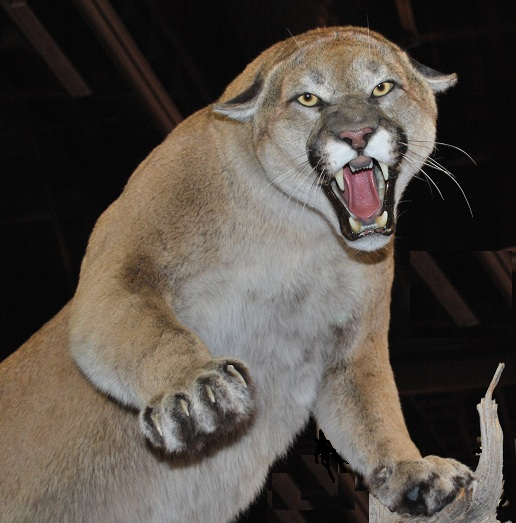
\includegraphics[width=3cm]{Cougar_Nevada}
\normalfont \normalsize 
%\textsc{APC 524} \\ [25pt] % Your university, school and/or department name(s)
\horrule{0.5pt} \\[0.4cm] % Thin top horizontal rule
\LARGE COUGAR (\textbf{CO}de \textbf{U}sually \textbf{G}enerates \textbf{A}xisymmetric \textbf{R}econstruction), \\ \Large An MHD Equilibrium Reconstruction Code: Final Report\\ % The assignment title
\horrule{2pt} \\[0.5cm] % Thick bottom horizontal rule
}

\author{Peter Bolgert (pbolgert@pppl.gov), Jonathan Ng (wng@pppl.gov), \\ Elizabeth Paul (epaul@princeton.edu), Jacob Schwartz (jschwart@pppl.gov)} % Your name

\date{\normalsize\today} % Today's date or a custom date

\begin{document}

\maketitle % Print the title

%----------------------------------------------------------------------------------------
%	Section 1
%----------------------------------------------------------------------------------------

\section{Project Objective / Summary}

Our goal was to write a program which solves the Grad-Shafranov equation (GSE) for axisymmetric plasmas in a user friendly manner.  The result is COUGAR, which stands for \textbf{CO}de \textbf{U}sually \textbf{G}enerates \textbf{A}xisymmetric \textbf{R}econstruction.  The main body of the code is written in C++, with a separate Python program for visualization.  The user can set code options either via the command line or text-based configuration file.  In the current version, simple analytic forms for pressure and toroidal magnetic field must be assumed.  Future versions of the code will deduce these quantities from experimental measurements.  For information on running COUGAR, see the user manual at \href{http://jonngwx.github.io/grad-shafranov/md__r_e_a_d_m_e.html}{\nolinkurl{jonngwx.github.io/grad-shafranov/md__r_e_a_d_m_e.html}}.

%----------------------------------------------------------------------------------------
%	Section 2
%----------------------------------------------------------------------------------------

\section{Theoretical Background}

\textbf{Notes}: The following material primarily follows Chapter 4 of \textit{Computational Methods in Plasma Physics}, by Stephen Jardin.  When there are discrepancies between that book and this document, the latter should be trusted as the former has misprints.  Also, SI units are used throughout.

\subsection{MHD equilibrium}

In magnetohydrodynamic (MHD) theory, a plasma equilibrium is described by the equation $\mathbf{\nabla} p = \mathbf{J} \times \mathbf{B}$, where $p$ is the scalar plasma pressure, $\mathbf{J}$ is the current density, $\mathbf{B} = \mathbf{\nabla} \times \mathbf{A}$ is the magnetic field, and $\mathbf{A}$ is the vector potential for the magnetic field.  We work in cylindrical coordinates $(R, \phi, z)$, and the plasma is assumed to be axisymmetric, i.e., $\partial / \partial \phi = 0$.

By introducing new functions $\Psi(R,z) \equiv -R A_{\phi}$ (called the flux function) and $g(R,z) \equiv R B_{\phi}$, we can rewrite the equilibrium equation in the following form, known as the Grad-Shafranov equation:
\begin{equation}
\Delta^{*} \Psi + \mu_0 R^2 \frac{dp}{d\Psi} + g \frac{dg}{d\Psi} = 0,
\end{equation}
where $\Delta^{*} \equiv R^2 \mathbf{\nabla} \cdot \frac{1}{R^2} \mathbf{\nabla}$ is called the toroidal elliptic operator. Here, $p(\Psi)$ and $g(\Psi)$ are functions of $\Psi(R,z)$, the quantity that we are trying to solve for.  Thus $p(\Psi)$ and $g(\Psi)$ must be given (along with boundary conditions) for the problem to be fully specified.  Once the equation is solved, any other quantity of interest ($\mathbf{J}$, $\mathbf{B}$, etc.) can be calculated.  

\begin{figure}
\centering
\captionsetup{justification=centering,margin=3cm}
\caption[caption]{Cylindrical coordinates $(R,\phi,z)$.  Taken from "Computational Methods in Plasma Physics," Stephen Jardin.}

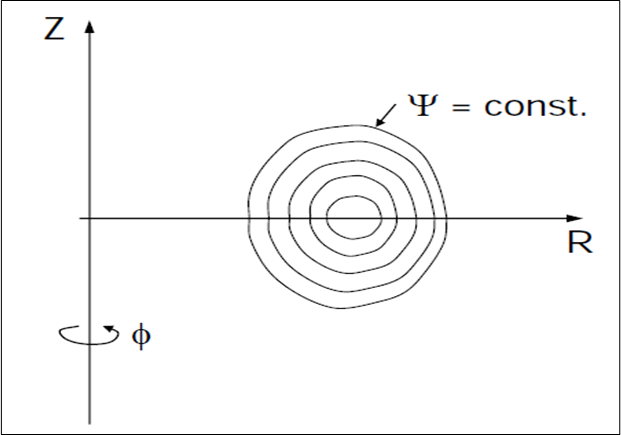
\includegraphics[width=0.35\textwidth]{coordinates}

\end{figure}

Without going into too much detail, it should be stated that the best MHD equilibria for confining plasmas are those which contain nested surfaces of constant $\Psi$ (known as flux surfaces), as in Figure 1.  It can be shown that a magnetic field line will always point tangentially to a given flux surface.  Since charged particles in the plasma follow field lines, the particles will stay on constant flux surfaces, resulting in good confinement. 



\subsection{Analytic Profiles vs Equilibrium Reconstruction}
As previously stated, the functions $p(\Psi)$ and $g(\Psi)$ must be supplied for a full specification of the problem.  In our code, we assumed simple analytic forms for these functions which roughly approximate real life experiments.  

Of course, in a real tokamak experiment, the functional forms of $g(\Psi)$ and $p(\Psi)$ are unknown.  Instead we must rely on a finite number of experimental measurements of $\Psi$ taken near the plasma boundary to deduce $p$ and $g$ as well as possible.  The approximate calculation of the flux function from these experimental measurements is known as Equilibrium Reconstruction, and will be implemented in a future version of COUGAR.  

\subsection{Algorithm when $p(\Psi)$ and $g(\Psi)$ are specified (current version of COUGAR)}

\textbf{Summary}: The problem is solved using a two-tiered iterative process.  The outer iteration (index $m$) determines the boundary values.  The inner iteration (index $n$) solves the GSE subject to those boundary conditions.
\\ \\
%%%%%% INNER ITERATION %%%%%%%%%%
\textbf{Detailed Steps}: First, rewrite the Grad-Shafranov equation as
\begin{equation}
\Delta^{*}\Psi = \mu_0 R J_{\phi} (R, \Psi),
\end{equation}
where $\mu_0 R J_{\phi} (R,\Psi) = - \big(\mu_0 R^2 \frac{d p}{d\Psi} + g \frac{d g}{d\Psi}\big)$, and $J_{\phi}$ is the current density in the $\phi$-direction.

\textbf{Inner Iteration}: Since the problem is nonlinear (the right-hand side of Eq.~(2) depends on $\Psi$), we use an iterative approach.  At each level of the inner iteration, we solve a finite difference version of 
\begin{equation}
\Delta^{*}\Psi^{n} = \mu_0 R J_\phi (R, \Psi^{n-1}),
\end{equation}
where $n$ denotes the iteration level. The solution of $\Psi^n$ is plugged into the right-hand side of Eq.~(3) for the next iteration.  This continues until the solution converges.  The linearized finite difference equation can be solved via a variety of methods, handled by base class \texttt{EllipticSolver}.  We currently have implemented two derived classes to solve Eq.~(3): the Gauss-Seidel method, and the method of Successive over-relaxation (SOR), which are explained in Section 3.  

At the very beginning of the calculation we must supply an initial guess of $J_{\phi}$.  We use a quadratic form of $J_{\phi}$ taken from a paper by Johnson et al.~(J.~Comp.~Phys.~32 (1979), 212-234).  It has several parameters which must be set, such as the total toroidal current $I_p$ (commonly called the plasma current).  See \texttt{gs\_solver.cc} for more information.

Next, we use the updated $\Psi^n$ to calculate the value of $\Psi$ at the plasma-vacuum boundary (this defines where we must set pressure and current to zero).  This calculation is handled by the \texttt{Critical} class, which is so named because the plasma boundary either exists at a saddle point of $\Psi$ (a critical point) or where the plasma touches a solid object, like the vessel wall. We use the terms ``plasma edge" and ``limiter" interchangeably in this document.  \texttt{Critical} also finds the magnetic axis, which is the point of minimum $\Psi$ (the center of the contours in Figure 1).  

Lastly in the inner iteration, we must update the current density $J_{\phi}$, handled by the base class \texttt{JSolver}.  As previously stated, the $\phi$-directed current density is given by $J_{\phi} = -R \frac{d p}{d \Psi} - \frac{1}{\mu_0 R} g \frac{d g}{d \Psi}$. Our most successful child class of \texttt{JSolver}, called \texttt{JSolverAlpha}, uses the following forms for $p$ and $g$:
\begin{subequations}
\begin{align}
	p(\Psi) &= p_0 \widetilde{\Psi}^{n_1},\\
          g^2(\Psi) &= g_0^2  \left[1 + \alpha_g \widetilde{\Psi}^{n_2} \right],
\end{align}
\end{subequations}
where $\widetilde{\Psi}$ is a normalized flux function defined by $\widetilde{\Psi} \equiv (\Psi_l - \Psi)/(\Psi_l - \Psi_0)$.  Here,  $\Psi_l$ and $\Psi_0$ are the $\Psi$-values at the plasma edge (limiter) and magnetic boundary, as determined by \texttt{Critical}.  In Eq.~(4), $p_0$ (the pressure at the magnetic axis), $g_0$ (related to the vacuum toroidal B-field), and the exponents $n_1,n_2$ must be specified on the command line or in a config file.  The parameter $\alpha_g$ is computed during each inner iteration so that the plasma current $I_p$ is conserved.   For the sake of self-containedness, here's the formula: $\alpha_g = \mu_0 \left[-p_0 \sum_{i,j} R_i n_1 \widetilde{\Psi}_{ij}^{(n_1-1)} + I_p (\Psi_l - \Psi_0)/dR\, dz \right] \bigg/ \left[\frac{1}{2} g_0^2 \sum_{i,j} n_2 \widetilde{\Psi}_{ij}^{(n_2-1)} / R_i\right]$, where $dR, dz$ are spaces between grid points.


%%% OUTER ITERATION %%%%%

\textbf{Outer Iteration}: The outer iteration deals with the nonlinearity due to boundary conditions.  Suppose that there are $N_{coils}$ external coils outside of the plasmal boundary (they can be inside or outside the computational grid).  The flux function evaluated on the computational boundary $\Psi(R',z')$ is then due to the plasma itself and the external coils:
\begin{equation}
\Psi^m (R',z') = \mu_0 \int_{plasma} G(R,z; R',z') J_{\phi}^{m-1} \mathop{dR} \mathop{dz} + \mu_0 \sum_{k=1}^{N_{coils}} G(R_k,z_k; R',z') I_k,
\end{equation}
where $G$ is the Green's function for the elliptic operator $\Delta^{*}$, $(R_k,z_k)$ is the location of the $k$th coil with current $I_k$, and $(R',z')$ refers to a point on the computational boundary. Here, $J_{\phi}^{m-1}$ is the converged current density from the previous  iteration.  The Green's function, which is defined by $\Delta^{*}G(\mathbf{R};\mathbf{R'}) = R \delta(R-R')\delta(z-z')$, is given by
\begin{equation}
G(\mathbf{R};\mathbf{R'}) = -\frac{1}{2\pi} \frac{\sqrt{RR'}}{k} [(2-k^2) K(k) - 2 E(k)], 
\end{equation} 
where $k^2 = 4RR'/[(R+R')^2+(z-z')^2]$, and where $K(k)$ and $E(k)$ are complete elliptic integrals as defined by the Boost special functions website (Arfken's book and Mathematica use slightly different definitions). The Green's function can be computed before the main calculation and stored in an array.


There is a faster method of calculating the boundary ($\mathcal{O}(N^2)$ vs $\mathcal{O}(N^3)$) known as Von Hagenow's method. It is described in Lackner, Comp.~Phys. Comm.~12 (1976) 33-44.  As the size of the grid increases, the time it takes to populate the Green's function array for Eq.~(5) can dominate the rest of the calculation.  The faster method needs a factor of $\approx N$ fewer Green's function values, making the calculation much quicker.    

Thus, given a set of boundary conditions, we can solve Eq.~(3) iteratively for $\Psi$.  This $\Psi$ is then used to calculate a new set of boundary conditions using Eq.~(5), and the process begins anew.  Ultimately, the process is a two-tiered iteration which runs until the outer loop converges.  The process is depicted in Figure 2.

\begin{figure}
\centering
\captionsetup{justification=centering,margin=3cm}
\caption[caption]{Double-nested iteration loop. Taken from "Computational Methods in Plasma Physics," Stephen Jardin.}
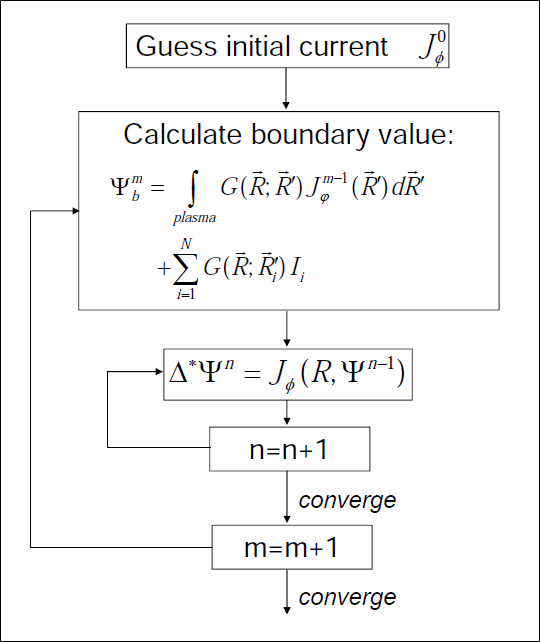
\includegraphics[width=0.45\textwidth]{algorithm}
\end{figure}

In summary, the \textbf{inputs} to the algorithm are an initial guess $J_\phi^0$ for the current density, the location of external coils $(R_k,z_k)$ and their currents $I_k$, and the functional forms of $p(\Psi)$ and $g(\Psi)$.  The \textbf{output} is the value of $\Psi$ at each grid point in the $R-z$ plane.  From there, any derived quantity can be calculated.  

\subsection{Algorithm using Experimental Measurements (for the future)}

In an experiment, $p(\Psi)$ and $g(\Psi)$ are unknown, but suppose we have $N_{meas}$ measurements of the flux function $\Psi_l^{meas}$ near the plasma boundary (but within the computational boundary).  

First we expand our unknown functions in terms of basis functions (e.g. Legendre polynomials):
\begin{equation}
p'(\Psi) = \sum_s \alpha_s y_s(\Psi), \quad gg'(\Psi) = \sum_s \beta_s y_s(\Psi).
\end{equation}
We can then write a formula for the computed value of $\Psi$ at the location $(R_l, z_l)$ of each experimental measurement: 
\begin{equation}
\Psi_l^{comp}(R_l, z_l) = \mu_0 \int_{plasma} G(R,z; R_l,z_l) J_\phi(R,\Psi,\alpha_s,\beta_s) dR dz + \mu_0 \sum_{k=1}^{N_{coils}} G(R_k ,z_k; R_l,z_l) I_k.
\end{equation}
The computed values are compared to the measured values, and the minimization of an error function determines the values of $\alpha_j, \beta_j$ at that stage in the algorithm.   

Thus, the algorithm described in Section 1.4 is identical to that described in Section 1.3 (and depicted in Fig.~2), except that each time $\Psi$ is updated in the inner ($n$) loop, we also update the values of $\alpha_s, \beta_s$.  In summary, the \textbf{inputs} to the algorithm are an initial guess $J_\phi^0$ for the source function, the location of external coils $(R_k,z_k)$ and their currents $I_k$, and the location of the experimental measurements $(R_l,z_l)$ and their values $\Psi_l^{meas}$.  The \textbf{output} is the value of $\Psi$ at each grid point in the $R-z$ plane.  



%----------------------------------------------------------------------------------------
%	Section 3
%----------------------------------------------------------------------------------------

\section{Code Organization / Class Structure}

The program is written in C++ with the visualization carried out separately using Python. The solver is called from the command line.  Options/parameters can be set on the command line or in a configuration file.  The location of external magnetic coils will also be contained in text files. Output will be written to text files or hdf5 files. 

The class structure of our code is explained in Table 1.  For more information, see the documentation website at \href{http://jonngwx.github.io/grad-shafranov/index.html}{\nolinkurl{jonngwx.github.io/grad-shafranov/index.html}}.

The following external libraries are used:
\begin{itemize}
\item HDF5 (version 1.8 or newer) is used for I/O. The libraries can be downloaded and installed from \texttt{www.hdfgroup.org}. Should the libraries be unavailable the program can be compiled and run with output written to a tsv file. 
\item Boost is used for the program options, math and testing libraries. 
\item The python numpy, h5py and matplotlib packages are used in our visualization program. 
\end{itemize}

%%%%%%%%%%%%%%%% BIG CLASS TABLE%%%%%%%%%%%%%%%%%
\newgeometry{left=0.1cm, right=0.1cm, top=0.1cm, bottom=0.35cm}
\begin{table}
\small
\tiny{\caption{Summary of COUGAR Classes (colors show class hierarchy)}}
\small
\centering
\begin{tabular}{ | m{2.8cm} | p{8.9cm} | p{6cm}|}
    \hline Class Name & Methods (inherited methods only listed in parent class) & Brief Description \\
    \hline Grid & 
\begin{lstlisting}[belowskip=-\baselineskip, aboveskip=-0.5\baselineskip]
double celli(double r)
double cellj(double z) 
\end{lstlisting} 
   & Stores information about the computational grid. \\
   \hline Field & none & Container for 2d data and the grid \\ 
   \specialrule{.05em}{0.0em}{.07em} \colorbox{blue!25}{EllipticSolver} & 
\begin{lstlisting}[belowskip=-\baselineskip, aboveskip=-0.5\baselineskip]
double norm_max (const Field &Psi, const Field &Psi_prev)
void iter(double omega)
void boundary (Field &Psi, const Field &Psi_prev) 
double norm()
virtual void step_1(const Field &jphi)=0
virtual void step(const Field &jphi)=0
virtual void coeff()=0
double residuals(const Field &Psi, const Field &Psi_prev) 
\end{lstlisting}
    &
    Base class for elliptic solvers like GaussSeidel and SOR which solve the finite difference GSE. 
     \\ 
    \specialrule{.05em}{0.0em}{.07em} \crule[blue!25]{0.35cm}{0.35cm} \, GaussSeidel &
\begin{lstlisting}[belowskip=-\baselineskip, aboveskip=-0.5\baselineskip]
void step_1(const Field &jphi)
void step(const Field &jphi)
void coeff()
\end{lstlisting} 
    & Derived class of EllipticSolver. Solves finite difference equation using Gauss-Seidel algorithm.\\
    \specialrule{.05em}{0.0em}{.07em}  \crule[blue!25]{0.35cm}{0.35cm} \, SOR & 
\begin{lstlisting}[belowskip=-\baselineskip, aboveskip=-0.5\baselineskip]
void step_1(const Field &jphi)
void step(const Field &jphi)
void coeff()
double omega()
\end{lstlisting}
    &Derived class of EllipticSolver.  Solves finite difference equation using Successive over-relaxation algorithm. \\ 
    \specialrule{.05em}{0.0em}{.07em} \colorbox{cyan!25}{JSolver} &
\begin{lstlisting}[belowskip=-\baselineskip, aboveskip=-0.5\baselineskip]
virtual void update(Field *jphi, Field *psi, Field *p, Field *g)=0
\end{lstlisting}
    & Base class of methods which calculate $J_{\phi}$ \\ 
    \specialrule{.05em}{0.0em}{.07em} \crule[cyan!25]{0.35cm}{0.35cm} \,JSolverAlpha &
\begin{lstlisting}[belowskip=-\baselineskip, aboveskip=-0.5\baselineskip]
void update(Field *jphi, Field *psi, Field *p, Field *g)
\end{lstlisting}
    &  Uses very simple forms of $p,g$ to calculate $J_{\phi}$. \\ 
    \specialrule{.05em}{0.0em}{.07em} \crule[cyan!25]{0.35cm}{0.35cm} \,JSolverNSTX & 
\begin{lstlisting}[belowskip=-\baselineskip, aboveskip=-0.5\baselineskip]
void update(Field *jphi, Field *psi, Field *p, Field *g)
\end{lstlisting}
    & Uses analytic forms of $p,g$ which resemble NSTX \\ 
    \specialrule{.05em}{0.0em}{.07em} \colorbox{green!25}{Boundary} & 
\begin{lstlisting}[belowskip=-\baselineskip, aboveskip=-0.5\baselineskip]
virtual int CalcB(Field *jphi)
int LtoI(int l)
int LtoJ(int l)
double norm()
\end{lstlisting}
    & 
    Base class of methods which calculate the boundary of $\Psi$.
     \\ 
    \specialrule{.05em}{0.0em}{.07em} \crule[green!25]{0.35cm}{0.35cm} \, SlowBoundary &
\begin{lstlisting}[belowskip=-\baselineskip, aboveskip=-0.5\baselineskip]
int CalcB(Field *jphi)
\end{lstlisting}
    & 
    Calculates bdy by integrating over $J_{\phi}$ and over the external coils.
    \\ 
     \specialrule{.05em}{0.0em}{.07em} \colorbox{orange!50}{Table} &
\begin{lstlisting}[belowskip=-\baselineskip, aboveskip=-0.5\baselineskip]
virtual int load_from_tsv(const string filename, int header_lines=0)
int num_columns() const
int num_rows() const
double data(int row, int column) const
\end{lstlisting}
    & Data format for 2d arrays of doubles and their metadata \\ 
    \specialrule{.05em}{0.0em}{.07em} \crule[orange!50]{0.35cm}{0.35cm} \, CoilData &
\begin{lstlisting}[belowskip=-\baselineskip, aboveskip=-0.5\baselineskip]
int load_from_tsv(const string filename, int header_lines=0) override
double r(int i) const
double z(int i) const
double current(int i) const
int num_coil_subregions() const
\end{lstlisting}
    & Container for the R and z location (m) and currents (A) of external coils. \\ 
    \hline Critical &
\begin{lstlisting}[belowskip=-\baselineskip, aboveskip=-0.5\baselineskip]
void Psi_search(double r, double z, double *dr, double *dz)
void Psi_magnetic(double r, double z, double *rcrit, 
	double *zcrit, double *Psi_min)
double Psi_limiter ()
void update ()
bool find_saddle (double &r, double &z)
\end{lstlisting}
    & 
    Finds `critical points' like the magnetic axis, limiter points, and X points.
     \\ 
    \hline Interpolate & 
\begin{lstlisting}[belowskip=-\baselineskip, aboveskip=-0.5\baselineskip]
double F (double r, double z) const
double F_r (double r, double z) const
double F_rr (double r, double z) const
double F_rz (double r, double z) const
double F_zz (double r, double z) const
double F_z (double r, double z) const
void updateInterpolation(double r, double z)
void PrintAmnCoefficients()
\end{lstlisting}
    & 
    Interpolates to find the values and derivatives of a 2D data set between grid points by fitting to a bicubic polynomial. 
     \\ 
    \specialrule{.05em}{0.0em}{.07em} \colorbox{magenta!25}{GradOutput} & 
\begin{lstlisting}[belowskip=-\baselineskip, aboveskip=-0.5\baselineskip]
virtual void write_output(const char *filename)=0
void parse_outputs(const char *outputs)
bool find(Output out)
\end{lstlisting}
    & Base class for writing the output of the solver to file. \\ 
    \specialrule{.05em}{0.0em}{.07em} \crule[magenta!25]{0.35cm}{0.35cm} GradOutputHdf & 
\begin{lstlisting}[belowskip=-\baselineskip, aboveskip=-0.5\baselineskip]
void write_output(const char *filename)
\end{lstlisting}
     & Writes data to a hdf5 file. \\ 
     \specialrule{.05em}{0.0em}{.07em} \crule[magenta!25]{0.35cm}{0.35cm} GradOutputTxt &
\begin{lstlisting}[belowskip=-\baselineskip, aboveskip=-0.5\baselineskip]
void write_output(const char *filename)
\end{lstlisting}
    & Writes data to a text file. \\ 
    \hline
\end{tabular}
\end{table}
%%%%%%%%%%%%%%% END BIG CLASS TABLE %%%%%%%%%%%%%%%

\restoregeometry

\subsection{Implementation and Design decisions}

\subsubsection{User Interface}
COUGAR is run from the Unix command line.  Options may be selected as command line options or specified in a configuration file.  We've provided a default configuration file (\texttt{grad-shafranov.cfg}) for your enlightenment.  The locations of external currents are specified in a specially formatted text file.  The default, called \texttt{coil\_data.tsv}, contains coil information from a particular NSTX shot.  

Once the code has run, the output may be viewed using a separate Python program. For much more on running COUGAR, please see the user manual on the documentation website.

\subsubsection{Elliptic solver}
The \texttt{EllipticSolver} interface defines functions for inverting the $\nabla^*$ operator iteratively using central finite differences, as shown in equation~\ref{eq:finitediff}.
\begin{multline} \label{eq:finitediff}
\frac{1}{R} \left(\frac{\Psi(R + dR, z) - \Psi(R - dR, z)}{2dR} \right) + \left( \frac{\Psi (R + dR, z) - 2\Psi(R,z) + \Psi(R-dR, z)}{dR^2} \right) \\ + \left(\frac{\Psi(R, z + dz) - 2\Psi(R,z)  + \Psi(R, z-dz)}{dz^2}\right) = \mu_0 R J_{\phi}(R,z). 
\end{multline}

Because the radial derivatives are $R$-dependent, the finite difference coefficients are stored as vectors. The successive over-relaxation (SOR) and Gauss-Seidel methods have been implemented, with Gauss-Seidel used in the current version of the code. While these algorithms are slow, they have been chosen as SOR can be parallelized, while Gauss-Seidel can be used as a starting point for multigrid methods. 

The Gauss-Seidel iteration method updates $\Psi^{n+1}_{i,j}$ using neighboring values of $\Psi^{n}$ and $\Psi^{n+1}$, 

\begin{multline} \label{eq:gaussseidel}
\Psi^{n+1}_{i,j} = -\frac{dR^2 dz^2}{2dz^2 + 2dR^2} \left[ \mu_0 R J^n_{\phi \, i, j} + \left(2 R dR - \frac{1}{dR^2}\right)^{-1} \Psi^{n}_{i+1,j} - \left(2 R dR - \frac{1}{dR^2}\right)^{-1} \Psi^{n+1}_{i-1,j} - \frac{1}{dz^2} \right] \Psi^{n+1}_{i,j-1} \\ - \frac{1}{dz^2}\Psi^n_{i, j+1}. 
\end{multline}

To aid with convergence we implement the Gauss Seidel algorithm with Picard iteration with $\alpha = 0.5$, 

\begin{equation} \label{eq:picard}
\Psi^{n+1} = \alpha_B \widehat{\Psi^{n+1}} + (1 - \alpha_{B}) \Psi^n, 
\end{equation}
where $\widehat{\Psi^{n+1}}$ is the tentative ``next" solution until the Picard iteration takes place.

The method of successive over-relaxation is based on the Gauss-Seidel method but has better convergence properties due to use of a strategically chosen blending parameter $\omega$: 

\begin{multline} \label{eq:SOR}
\Psi^{n+1}_{i,j} = (1-\omega)\Psi^n_{i,j} -\frac{\omega dR^2 dz^2}{2dz^2 + 2dR^2} \left[ \mu_0 R J^n_{\phi \, i, j} + \left(2 R dR - \frac{1}{dR^2}\right)^{-1} \Psi^{n}_{i+1,j} - \left(2 R dR - \frac{1}{dR^2}\right)^{-1} \Psi^{n+1}_{i-1,j} - \frac{1}{dz^2} \right] \Psi^{n+1}_{i,j-1} \\ - \frac{1}{dz^2}\Psi^n_{i, j+1}
\end{multline}

where
\begin{equation}
\omega = \frac{2}{1 + \sqrt{1 - \delta}}
\end{equation}
\begin{equation}
\delta = \frac{\text{max} (\left| \Psi^n - \Psi^{n-1} \right| )}{\text{max} (\left| \Psi^{n+1} - \Psi^{n} \right| )}.
\end{equation}

\subsubsection{Current density calculations}
The calculation of $P$, $gg'$ and $J_\phi$ is performed by the implementation of the \texttt{JSolver} interface. $P$ and $g$ are assumed to be functions of $\Psi$ from which the current density $J_\phi$ is calculated. The default \texttt{JSolverAlpha} uses a constant $P'$ and a linear $gg'$, with the coefficients of the functional forms determined by the peak pressure and the total current in the plasma. The exact exponent on $\Psi$ can be modified by changing $n_1$ and $n_2$ in the input or configuration file. \texttt{JSolverNSTX} attempts to use similar functional forms to the actual NSTX data.  It uses a quadratic $P'$ and $gg' = \sum_n A_n\Psi^n$, but there are numerical issues with maintaining the zero gradient condition at the plasma edge. As such, its use is not recommended in the current version. 

If experimental measurements of $\Psi$ were added to the code, the functional dependence on $\Psi$ of $P$ and $g$ would be determined by performing a least-squares fit to the data. 

\subsubsection{Output}
All the output is done through the \texttt{GradOutput} interface, with options to write to hdf or tsv files. As only $\Psi$, $P$ and $g$ are necessary for the solution of the equation, the default output writes only these three quantities and the dimensions of the grid. The value of the flux function $\Psi$ at the limiter and magnetic axis are also written to identify the plasma position. In the tsv case, this is an additional quantity while in the hdf version, this is an attribute of the \texttt{psi} dataset. These formats were chosen because ASCII can be read and written easily and should work on most systems, while HDF5 is a standard data structure for scientific work. Output can be written during the calculation if desired.

Additional quantities are added to the output by passing a comma separated string to the constructor, which is parsed. Currently, options for the toroidal current density and toroidal magnetic field are available, though additional output fields can be added by modifying the parsing function and adding the appropriate quantity to the writing function. Additional output formats can be added by implementing the \texttt{GradOutput} interface.

\subsubsection{Visualization}

The python visualizer can be run from command line or interactively. The data are read using the \texttt{read\_data} module, which passes a dictionary of the available fields to the plotting function in the \texttt{viz} module. Tsv data are read using regular expressions while HDF data are read using functions provided by \texttt{h5py}. In the command line version, contour and color plots of $\Psi$, $P$ and $g$ are shown in a single figure and the matplotlib \texttt{format\_coord} function is overridden so the values of the data can be read off the figure. An additional function is provided to produce a radial plot of the values of a field along the midplane of the tokamak. 

The use of a dictionary to hold the data was chosen in order to make reading the output files more convenient; we can simply iterate over the lines of the tsv output or datastructs of the HDF file. Also, with the option to add custom outputs, checking for the existence of each field would have to be performed while reading. The disadvantage of this approach is that referring to the data is unwieldy (\texttt{F['R']} vs \texttt{F.R} for example). An example of the output, which looks similar to an NSTX plasma, is shown in Fig.~\ref{fig:eqm}

\begin{figure}
	\centering
	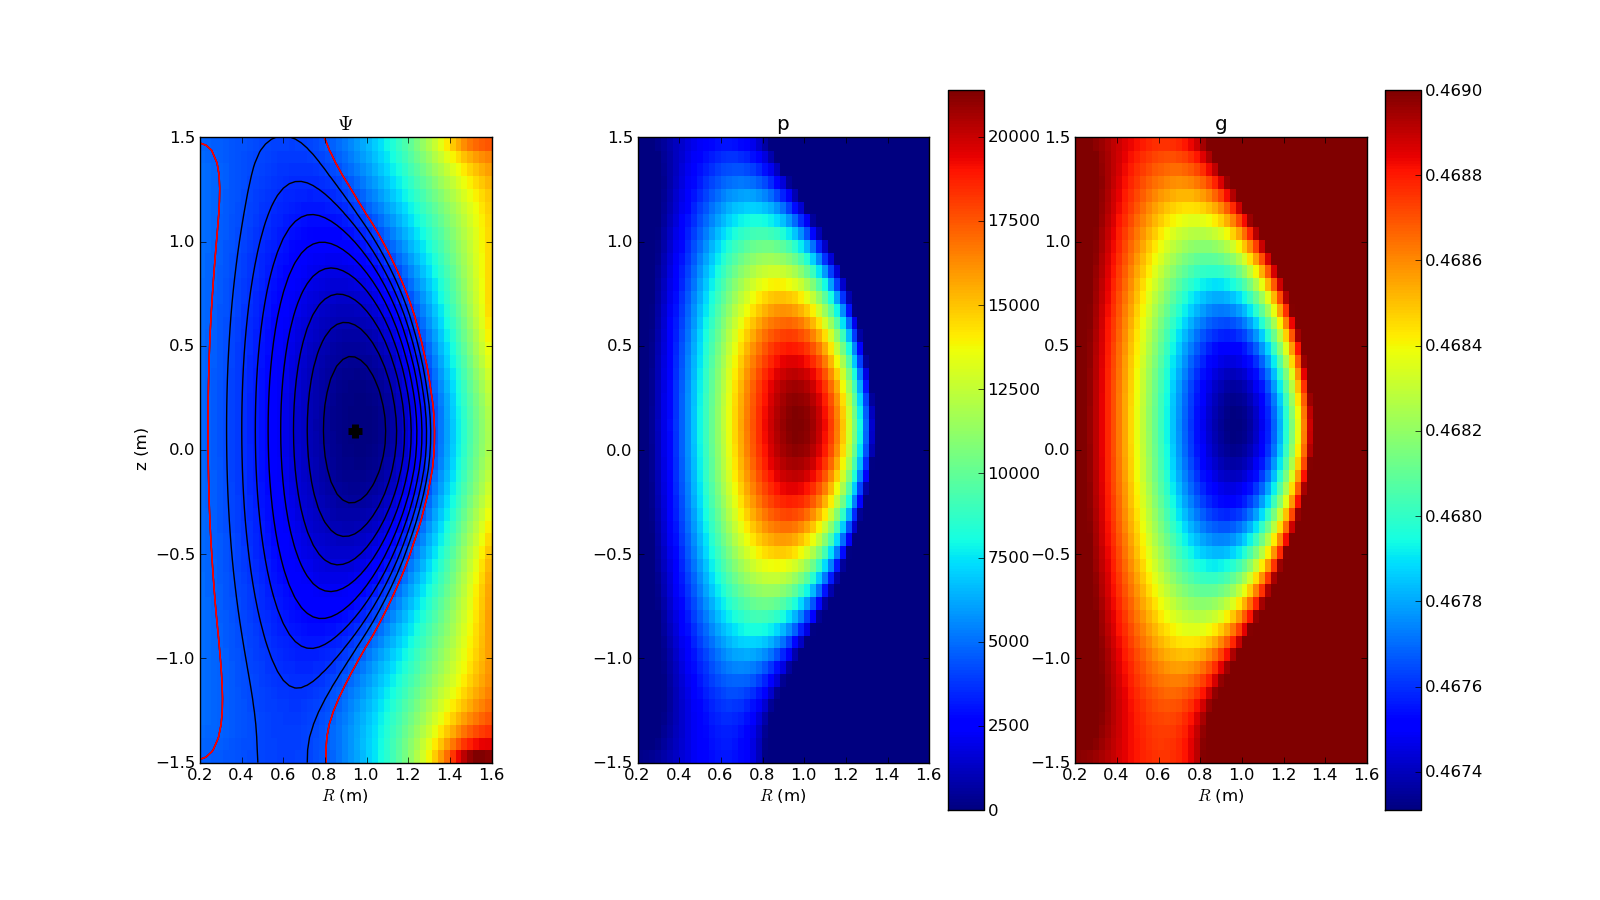
\includegraphics[width=0.8\textwidth]{eqm}
	\caption{Output of the Grad-shafranov solver. From left to right, $\Psi$, pressure and $g$. }
	\label{fig:eqm}
\end{figure}


%----------------------------------------------------------------------------------------
%	Section 4
%----------------------------------------------------------------------------------------

\section{Testing}

We have used the Boost Unit Test framework for testing of all major classes. The \texttt{EllipticSolver} class has been tested by comparison to the multipole expansion of the vacuum solution, $\nabla^* \Psi = 0$. As $J_{\phi} = 0$, only the inner loop needs to be iterated over. The \texttt{Elliptic} class is also tested by comparison to the analytic Shafranov-Solov\'ev solution. The \texttt{Interpolate} class is tested by comparison to interpolated linear and quadratic functions. The \texttt{SlowBoundary} class is tested by checking for the consistency of green\_fcn.cc, \texttt{SlowBoundary}, and \texttt{GaussSeidel} using the Shafranov-Solov\'ev solution. Test suites have also be written for \texttt{Boundary}, \texttt{Grid}, the tsv reader, and other utility functions.

Throughout the project, we tested for memory leaks using Valgrind.

%----------------------------------------------------------------------------------------
%	Section 5
%----------------------------------------------------------------------------------------

\section{Profiling}

In order to determine the runtime scaling we ran gs\_solver using the default configuration file, only changing the grid size. We ran from 32x32 through 80x80 every 5 (we would have done 30x30 but the physical positions of the limiters are too close to the computational boundary for grids smaller than 32x32). Only for the 32x32 case were there no errors (from Interpolate, about a wrong grid cell, from the main solver, about the $m$ iterations maximum limit reached, or from Critical not finding a critical point properly). Most of the other runs hit the maximum $m$ limit and when plotted showed the plasma had drifted unphysically upwards. Every run required different numbers of inner $n$-iterations to converge (this explains some of the scatter in the main-solve timing data).

In order to time the run we used <time.h> and clock(): first to time the setup (calculating the array of Green's function values) and then to time the main solver loop (iterations over $m$ and $n$). In the figure, setup time is the blue dots and the solver time is the black dots. In dashed lines are simple polynomial fits to these data: $t = a N^b$ where $t$ is time, $N$ is grid size, and $a$ and $b$ are the coefficients to be fitted to the data. For the setup $b \approx 2.4$ with fairly small scatter, and for the main loop $b \approx 3.7$.

\begin{figure}
	\centering
	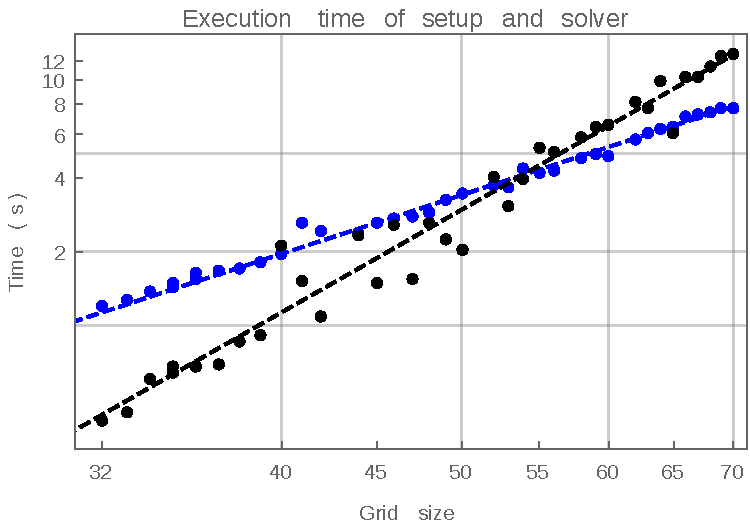
\includegraphics[width=0.6\textwidth]{run_times.pdf}
	\caption{Plot of wall time vs grid size for the \textcolor{blue}{\textbf{setup}} stage of the calculation (blue dots) and the \textbf{solver} stage (black dots).  The setup goes like $\approx \mathcal{O}(N^{2.4})$ and the solver goes like $\approx \mathcal{O}(N^{3.7})$.}
\end{figure}

We also used kcachegrind. When we ran with a 50x50 grid it appeared that more time was spend in the solver (GaussSeidel) than the setup (SlowBoundary): about 60\%/40\% vs the opposite ratio for that size from the bare timing with clock(). 

%----------------------------------------------------------------------------------------
%	Section 6
%----------------------------------------------------------------------------------------

\section{Lessons Learned/ Miscellaneous}
\subsection{Lessons Learned}

We all greatly improved in our C++ skills during this project.  Most of us came into this class more familiar with scripting languages like Matlab or Python.  As the project progressed, we also grew more comfortable with Git.  I can't imagine doing a project like this without it.  We ended up making over 600 commits!  We also learned that solving the Grad-Shafranov equation is a highly nonlinear and nontrivial problem.  Depending on the parameters you choose, our iterations often go unstable or converge to very strange solutions.  

For future generations of APC524, we advise that you fully understand your algorithms before writing code.  Otherwise, you'll have to rewrite most of it later!  

\subsection{Miscellaneous}
Breakdown of labor:

\begin{itemize}
\item Peter: Boundary classes, JSolver classes, Green's Functions
\item Jonathan: Output, Visualization 
\item Elizabeth: EllipticSolver classes, Interpolate, Critical (with Jonathan)
\item Jacob: Input, CoilData, Doxygen (helped by all)
\end{itemize}

\end{document}
